\documentclass{ximera}

\addPrintStyle{../..}

\begin{document}
	\author{Bart Lambregs}
	\xmtitle{Bewerkingen met vectoren}{}
    \xmsource\xmuitleg


% SCALAIRE VERMENIGVULDIGING 

% ph: maar met 1 shift vector doen; is veel simpelen -1*(Shift) is de andere
%  TIKZPICTURE DIE DE SCALAIRE VERMENIGVULDIGING ILLUSTREERT 

\subsection*{Scalaire vermenigvuldiging van een reëel getal met een vector}


Een vector kan 'herschaald' worden door hem te vermenigvuldigen met een reëel getal (d.w.z. een scalar). De richting blijft op die manier behouden. 
De grootte en zin kunnen veranderen. 
De scalaire verminigvuldiging wordt genoteerd als \(\vec{c} = k \cdot \vec{a}\) waarbij \(k \in \R\).

% ERUIT OP AANRADEN VAN VINCENT: 
% Als de vector \(\vec{a}\) gegeven wordt door \((a_x, a_y)\), is de scalaire vermenigvuldiging \(3\cdot\vec{a}\) gelijk aan \(3\cdot((a_x, a_y)) = (3a_x, 3a_y)\).

% Het is een soort reëel veelvoud van de vector. 

\begin{image}[0.3\textwidth]
\begin{tikzpicture}
    % \draw (-4,-4) grid (4,4);

    \pgfmathsetmacro{\ax}{2}  
    \pgfmathsetmacro{\ay}{0.5}  

    % \pgfmathsetmacro{\c}{$\sqrt{2}$}  
    \pgfmathsetmacro{\d}{2} 

    \coordinate (O) at (0,0); 
    \coordinate (A) at (\ax,\ay); 
    
    \coordinate (Shift) at (0,0.1); 

    \fill (O) circle (2pt); %node[below left]{O};

    \draw[->, very thick,  -latex] (O) -- ($(A)$) node[midway, below]{\(\vec{a}\)};
    \draw[->, very thick,  -latex, blue] ($ (O) - (Shift)$) -- ($-1*(A) - (Shift)$) node[midway, above]{\(-\vec{a}\)};

    \draw[->, very thick,  -latex] ($ (O) + (Shift)$) -- ($\d*(A) + (Shift)$) node[midway, above]{\(2 \cdot \vec{a}\)};
    \draw[->, very thick,  -latex, blue] ($ (O) - 2*(Shift)$) -- ($-0.5*(A) - 2*(Shift)$) node[midway, below]{\(-\frac{1}{2}\vec{a}\)};

\end{tikzpicture}
\end{image}
\captionof{figure}{De scalaire vermenigvuldiging van een vector \(\vec{a}\)}



\subsection*{De samenstelling of som van twee (of meer) vectoren}

Twee vectoren van dezelfde grootheid met hetzelfde aangrijpingspunt kunnen opgeteld worden met als resultaat een nieuwe vector. 
Deze vector wordt \textbf{de resultante} genoemd. 
Grafisch (kwalitatief) bekomt men de resultante via de kopstaartmethode of parallellogrammethode.  %kopstaartmethode (voor de eenvoud enkel parallellogram gebruiken? --> toch niet (vincent))

\begin{image}[0.4\textwidth]
    \begin{tikzpicture}
     % TIKZPICTURE DIE DE SOM VAN TWEE VECTOREN BEREKENT 
    % \draw (-4,-4) grid (4,4);

    \pgfmathsetmacro{\ax}{1}  
    \pgfmathsetmacro{\ay}{2}  
    \pgfmathsetmacro{\bx}{3}  
    \pgfmathsetmacro{\by}{1} 

    \coordinate (O) at (0,0); 
    \coordinate (A) at (\ax,\ay); 
    \coordinate (B) at (\bx,\by); 

    \fill (O) circle (2pt) node[below left]{O};
    % \fill (A) circle (2pt);
    % \fill (B) circle (2pt);

    \draw[->, -latex] (O) -- (A) node[midway, below]{\(\vec{a}\)};
    \draw[->, -latex] (O) -- (B) node[midway, below]{\(\vec{b}\)};
    
    \draw[->, -latex, red, thick] (O) -- ($ (A) + (B)$) node[midway, below]{\(\vec{a} + \vec{b}\)};
    \draw[->, dashed, -latex, red, thick] (A) -- ($ (A) + (B)$) node[midway, below]{\( \vec{b} \)};
    \draw[->, dashed, -latex, red, thick] (B) -- ($ (A) + (B)$) node[midway, below]{\( \vec{a} \)};

\end{tikzpicture}
\end{image}
\captionof{figure}{De optelling van twee vectoren}


De \textbf{grootte van de resultante} (kwantitatief) kan op verschillende manieren bepaald worden. 
Erg belangrijk hierbij is om meetkundige samenstelling in het oog te houden en zeker niet blindelings de groottes van de gegeven vectoren op te tellen! 
In het algemeen wordt de grootte van de resultante berekend met de cosinusregel. 
In evenwijdige of loodrechte gevallen zijn er efficiënte manieren om de resultante te bepalen (som/verschil of stelling van Pythagoras), de meest algemene methode is echter met de (gewijzigde) cosinusregel:

\[
\vec{c} = \vec{a} + \vec{b} \Rightarrow \| \vec{c} \|^2 = \| \vec{a} \|^2 + \| \vec{b} \|^2 + 2 \cdot \|\vec{a}\| \cdot \|\vec{b}\| \cdot \cos(\alpha)
\]

met \(\alpha\) de hoek tussen \(\vec{a}\) en \(\vec{b}\). 

\begin{quickquestion*}{}{}
  Hoe vereenvoudigt de formule als \(\vec{a}\) en \(\vec{b}\) loodrecht staan? Wat als ze dezelfde richting hebben? 
\end{quickquestion*}

\begin{example}

In onderstaande figuur is \(\|\vec{a}\| = \SI{3}{\newton}\) en \(\|\vec{b}\| = \SI{5}{\newton}\). 
Bijgevolg is  \(\| \vec{c} \| = \|\vec{a}\| + \|\vec{b}\| = \SI{8}{\newton}\). 

\begin{image}[0.3\textwidth]
    \begin{tikzpicture}
        \coordinate (O) at (0,0);
        \coordinate (A) at (1,0);
        \coordinate (B) at (2,0);
        \coordinate (C) at (3,0);

        \coordinate (Shift) at (0,0.05);

        \fill[xmgreen] (O) circle (1pt);
        \fill[red] ($ (O) + (Shift) $) circle (1pt);
        \fill[blue] ($ (O) - (Shift) $) circle (1pt);


        \draw[->, red] ($ (O) + (Shift) $)--($ (A) + (Shift) $)  node[midway, above]{$\vec{a}$};
        \draw[->, xmgreen] (O)--(C)                                  node[pos=0.7, above]{$ \vec{c} = \vec{a} + \vec{b} $};
        \draw[->, blue] ($ (O) - (Shift) $)--($ (B) - (Shift) $)  node[midway, below]{$\vec{b}$};
    \end{tikzpicture}
\end{image}
\end{example}

\begin{example}

% hier staat onnauwkeurigheid; de norm moet buiten de bewerking staan; de norm van een verschil is commutatief

In onderstaande figuur is \(\|\vec{a}\| = \SI{3}{\newton}\) en \(\|\vec{b}\| = \SI{5}{\newton}\). 
Bijgevolg is  \(\| \vec{c} \| = \|\vec{a} + \vec{b}\| =  \SI{5}{\newton} - \SI{3}{\newton}  = \SI{2}{\newton}\). 

\begin{image}[0.3\textwidth]
    \begin{tikzpicture}
        \coordinate (O) at (0,0);
        \coordinate (A) at (-1,0);
        \coordinate (B) at (2,0);
        \coordinate (C) at (1,0);

        \coordinate (Shift) at (0,0.05);

        \fill[xmgreen] (O) circle (1pt);
        \fill[red] ($ (O) + (Shift) $) circle (1pt);
        \fill[blue] ($ (O) - (Shift) $) circle (1pt);


        \draw[->, red] ($ (O) + (Shift) $)--($ (A) + (Shift) $)  node[midway, above]{$\vec{a}$};
        \draw[->, xmgreen] (O)--(C)                                node[pos=0.7, above]{$ \vec{c} = \vec{a} + \vec{b} $};
        \draw[->, blue] ($ (O) - (Shift) $)--($ (B) - (Shift) $) node[midway, below]{$\vec{b}$};
    \end{tikzpicture}
\end{image}
\end{example}



\begin{example}

In onderstaande figuur is \(\|\vec{a}\| = \SI{3}{\newton}, \; \|\vec{b}\| = \SI{5}{\newton} \text{ en } \alpha = 50^\circ\). 

    \begin{image}[0.5\textwidth]
        \begin{tikzpicture}
            % TIKZPICTURE DIE DE SOM VAN TWEE VECTOREN BEREKENT 
           % \draw (-4,-4) grid (4,4);
       
        %    \pgfmathsetmacro{\ax}{1}  
        %    \pgfmathsetmacro{\ay}{2}  
        %    \pgfmathsetmacro{\bx}{3}  
        %    \pgfmathsetmacro{\by}{1} 

           \pgfmathsetmacro{\ang}{50} 
       
           \coordinate (O) at (0,0); 
           \coordinate (A) at (\ang :2); 
           \coordinate (B) at (0:3); 
           \coordinate (C) at ($ (A) + (B)$); 
           
           \coordinate (Z) at (180:1); 

           \draw[dotted] (O)--(Z);
       
           \draw[->, -latex, blue] (O) -- (A) node[midway, above left]{\(\vec{a}\)};
           \draw[->, -latex, red] (O) -- (B) node[midway, below]{\(\vec{b}\)};
           \draw[->, -latex, xmgreen] (O) -- (C) node[pos=1, above right, xmgreen]{\(\vec{c} = \vec{a}+\vec{b}\)};
           
           \draw[->, dashed, -latex, red, thick] (A) -- (C) node[midway, above left]{\( \vec{b} \)};
           \draw[->, dashed, -latex, blue, thick] (B) -- (C) node[midway, below right]{\( \vec{a} \)};

           \draw pic[ pic text = \(\alpha\), draw, angle radius=0.4cm]{angle= B--O--A};
           \draw pic[ pic text = \(\gamma\), draw, angle radius=0.7cm, angle eccentricity=1.2]{angle= B--O--C};
           \draw pic[ pic text = \(\varphi\), draw, angle radius=0.5cm]{angle= C--B--O};
           \draw pic[ pic text = \(\varphi\), draw, angle radius=0.5cm]{angle= A--O--Z};
       \end{tikzpicture}
    \end{image}
    
De grootte van de resultante \(\vec{c}\) wordt bepaald met de cosinusregel: 

% Cosinusregel
\[
\|\vec{c}\|^2 = \|\vec{a}\|^2 + \|\vec{b}\|^2 - 2 \,\|\vec{a}\|\,\|\vec{b}\|\cos\varphi
\]
\[
= \|\vec{a}\|^2 + \|\vec{b}\|^2 - 2 \,\|\vec{a}\|\,\|\vec{b}\|\cos(180^\circ - \alpha)
\]
\[
= \|\vec{a}\|^2 + \|\vec{b}\|^2 - 2 \,\|\vec{a}\|\,\|\vec{b}\|(-\cos\alpha)
\]
\[
= \|\vec{a}\|^2 + \|\vec{b}\|^2 + 2 \,\|\vec{a}\|\,\|\vec{b}\|\cos\alpha
\]
\[
= \sqrt{3^2 + 5^2 + 2 \cdot 3 \cdot 5 \cdot \cos 50^\circ} \approx \SI{7.3}{N}. 
\]

\end{example}

\begin{remark}
In het algemeen geldt dus \textbf{niet} dat \(\|\vec{c}\| = \| \vec{a+b}\| = \|\vec{a}\| + \|\vec{b}\|\). In welk(e) geval(len) geldt de eigenschap wel? 
\end{remark}


De \textbf{richting van de resultante} (d.w.z. de hoek \(\gamma\)) kan bepaald worden met de sinusregel: 

% TODO HIER IS GEEN COMMANDO \BGSIN 

\[
\frac{\sin\gamma}{\|\vec{b}\|} = \frac{\sin\alpha}{\|\vec{c}\|}
\quad\Longrightarrow\quad
\sin\gamma = \frac{\|\vec{b}\|\sin\alpha}{\|\vec{c}\|}
\]
\[
\gamma = \bgsin\!\left(\frac{5\cdot\sin 50^\circ}{7.3}\right) \approx 18^\circ
\]



% TODO;  TIKZ VAN SOM HERNEMEN MET GROOTTE EN RICHTING RESULTANTE OP AANGEDUID 


De optelling van vectoren is \textit{associatief}, d.w.z. dat \((\vec{a} + \vec{b}) + \vec{c} = \vec{a} + (\vec{b} + \vec{c})\). 
Met deze eigenschap kan je de som bereken van meerderen vectoren. 
Indien er dus meer dan twee vectoren worden samengesteld, tel je eerst twee ervan met elkaar op en het resultaat daarvan tel je met de volgende op, enzovoort totdat alle vectoren in de som zitten (zoals ook met de optelling van getallen gebeurt)

\subsection*{Verschil van twee vectoren}

Net zoals bij getallen is het ook mogelijk voor vectoren om van een verschil een som te maken: 

\[
\vec{c} = \vec{a}-\vec{b} = \vec{a} + (-\vec{b})
\]

Om \(\vec{c}\) te vinden moeten \(\vec{a}\) en \(-\vec{b}\) dus worden samengesteld.
Het verschil van de getallen acht en vijf is gelijk aan drie. 
Drie is dus het getal dat je bij vijf moet optellen om acht te bekomen. 
Op dezelfde manier is het verschil van vectoren \(\vec{a}\) en \(\vec{b}\) gelijk aan de vector \(\vec{c}\) die je bij \(\vec{b}\) moet optellen om \(\vec{a}\) te bekomen.
 \(\vec{c}\)is dus inderdaad het verschil of 'onderscheid' tussen \(\vec{a}\) en \(\vec{b}\). 


% TIKZPICTURE DIE HET VERSCHIL VAN TWEE VECTOREN WEERGEEFT 
\begin{image}[0.5\textwidth]
    \begin{tikzpicture}
        \pgfmathsetmacro{\r}{3}
        \pgfmathsetmacro{\ra}{0.5 * \r}
        \pgfmathsetmacro{\ang}{50}

        \coordinate (O) at (0:0);
        \coordinate (A) at (\ang : \ra);
        \coordinate (B) at (0:\r);
        \coordinate (minB) at (180:\r);
        
        \draw[->, -latex, blue   ] (O)--(A) node[midway, above left]{$\vec{a}$};
        \draw[->, -latex, red    ] (O)--(B) node[midway, below]{$\vec{b}$};
        \draw[->, -latex, xmgreen] (B)--(A) node[midway, above right]{$\vec{c}$};
        \draw[->, -latex, red    ] (O)--(minB) node[midway, below]{$-\vec{b}$};
        \draw[->, -latex, xmgreen] (O)--($(A) - (B)$) node[midway, above right]{$\vec{c}$};
        
        \draw[dotted] (A)--($(A) - (B)$)--(minB);
        \fill[red] (O) circle (1pt); 
    \end{tikzpicture}
\end{image}
\captionof{figure}{Het verschil van de vectoren $\vec{a}$ en $\vec{b}$}

Grafisch blijkt dat indien \(\vec{a}\) en \(\vec{b}\) in hetzelfde punt aangrijpen, \(\vec{a} - \vec{b}\) gelijk is aan de vector met als aangrijpingspunt het eindpunt van \(\vec{b}\) en als eindpunt het eindpunt van \(\vec{b}\).


% TODO: VINCENT HEEFT NOG EEN VOORBEELD VAN DE SLIDES HIER EXTRA GEGEVEN TIJDENS REVIEUW

\subsection*{De loodrechte ontbinding of projectie van een vector in componenten}


% dit zou iets uitgebreiden moeten via de omgekeerde richting (een vecor is eerder opgebouwd uit zijn componenten)

Een vector is opgebouwd als de samenstelling van zijn componten volgens de assen.  
In bepaalde contexten is het vaak erg nuttig om een vector (loodrecht) te ontbinden in zijn componenten. 
Noteer met \(\vec{a}_x\) de component volgens de \(x\)-as en met \(\vec{a}_y\) de component volgens de \(y\)-as. 
Voor elke vector geldt dan 
\[
\vec{a} = \vec{a}_x + \vec{a}_y
\]

De grootte van de componenten volgt rechtstreeks uit de goniometrische getallen: 

\[
\cos(\alpha) = \frac{\| \vec{a}_x \|}{\| \vec{a} \|} \Rightarrow \| \vec{a}_x \| = \|\vec{a}\| \cdot \cos(\alpha)
\]

\[
\sin(\alpha) = \frac{\| \vec{a}_y \|}{\| \vec{a} \|} \Rightarrow \| \vec{a}_y \| = \|\vec{a}\| \cdot \sin(\alpha)
\]

% TIKZPICTURE DIE DE ONTBINDING IN COMPONENTEN WEERGEEFT 
\begin{image}[0.3\textwidth]
\begin{tikzpicture}
    % \draw (-4,-4) grid (4,4);

    \pgfmathsetmacro{\ax}{1}  
    \pgfmathsetmacro{\ay}{2}  

    \coordinate (O) at (0,0); 
    \coordinate (A) at (\ax,\ay); 
    \coordinate (AX) at (\ax,0); 
    \coordinate (AY) at (0,\ay); 

    \fill (O) circle (2pt) node[below left]{O};

    \draw[->, -latex] (O) -- (A) node[midway, below]{\(\vec{a}\)};
    \draw[->, dashed, -latex, red, thick] (O) -- (AX) node[midway, below]{\( \vec{a}_x \)};
    \draw[->, dashed, -latex, red, thick] (O) -- (AY) node[midway, left]{\( \vec{a}_y \)};
    \draw pic[ pic text = \(\alpha\), draw, angle radius=0.4cm]{angle= AX--O--A};

    \draw[dotted] (0,\ay)--(A)--(\ax,0);
\end{tikzpicture}
\end{image}
\captionof{figure}{De loodrechte projectie van de vector \(\vec{a}\)}

Indien de componenten worden geschreven met behulp van de basisvectoren geeft dit 


$$
\vec{a} = \vec{a}_x + \vec{a}_y = a_x \cdot \vec{e}_x + a_y \cdot \vec{e}_y 
$$

% VINCENT: KIER KAN NOG EEN EXTRA FABEELDIN G

\subsection*{Het scalair product van twee vectoren (of inwendig product)}

Twee vectoren kan men op twee verschillende manieren met elkaar vermenigvuldigen die een ander resultaat opleveren. 

Het scalair product levert een \textbf{scalar} (= getal) als resultaat op die per definitie gelijk is aan de grootte van de projectie van de ene vector op de andere vermenigvuldigd met de grootte van diezelfde andere vector. 

Het scalair product wordt alsvolgt gedefineerd: 

% todo: hier gedefineerd als? 
$$
c = \vec{a} \cdot \vec{b} = \| \vec{a}_x \| \cdot \|\vec{b}\| = \|\vec{a}\| \cdot \cos(\alpha) \cdot \|\vec{b}\| = \| \vec{a}\| \cdot \| \vec{b}\| \cdot \cos(\alpha)
$$

\begin{quickquestion*}{}{}
    Is de eerste bewerking '\(\cdot\)' dezelfde als de tweede bewerking '\(\cdot\)'? Verklaar. 
\end{quickquestion*}

% TIKZPICTURE DIE SCALAIR PRODUCT van a op b ILLUSTREERT  
\begin{image}
\begin{tikzpicture}
    % \draw (-4,-4) grid (4,4);

    \pgfmathsetmacro{\ax}{1}  
    \pgfmathsetmacro{\ay}{2}  
    \pgfmathsetmacro{\bx}{3}  
    \pgfmathsetmacro{\by}{0} 

    \coordinate (O) at (0,0); 
    \coordinate (A) at (\ax,\ay); 
    \coordinate (B) at (\bx,\by); 

    \fill (O) circle (2pt) node[below left]{O};
    
    \draw[->, -latex] (O) -- (B) node[midway, below]{$\vec{b}$};

    \draw[->, -latex] (O) -- (A) node[midway, above left]{$\vec{a}$};
    \draw[->, dashed, -latex, red, thick] (O) -- (\ax, 0) node[midway, below]{$ \vec{a}_x $};
    \draw[dashed, -latex, thick] (\ax, 0) -- (A);


    \draw pic[ pic text= $\alpha$, draw,  angle radius=0.7cm]{angle = B--O--A}; 
\end{tikzpicture}
\end{image}
\captionof{figure}{De projectie van de vector $\vec{a}$ op $\vec{b}$}

\subsection*{Het vectorieel product van twee vectoren (of kruisproduct)}

Het vectorieel product levert een \textbf{vector} als resultaat op waarvan de grootte gelijk is aan de oppervlakte van de parallellogram ingesloten tussen de twee vectoren. 
De richting van het vectorproduct is loodrecht op het vlak gevormd door de twee gegeven vectoren en de zin is te bepalen met de rechterhandregel.
Het vectorieel product wordt genoteerd als 

\[
\vec{c} = \vec{a} \times \vec{b} = \| \vec{a}_y \| \cdot \|\vec{b}\| = \|\vec{a}\| \cdot \sin(\alpha) \cdot \|\vec{b}\| = \| \vec{a}\| \cdot \| \vec{b}\| \cdot \sin(\alpha)
\]

\begin{image}[0.4\textwidth]
    \begin{tikzpicture}
        
        \pgfmathsetmacro{\ax}{1}
        \pgfmathsetmacro{\ay}{2.2}
        \pgfmathsetmacro{\bx}{1.8}
        \pgfmathsetmacro{\by}{0}

        \coordinate (O) at (0,0);
        \coordinate (A) at (\ax,\ay);
        \coordinate (B) at (\bx,\by);

        \fill[gray!50] (O)--(A)--($(A)+(B)$)--(B)--cycle;

        \draw[->, -latex, blue] (O)--(A) node[midway, above left]{$\vec{a}$};
        \draw[->, -latex, red] (O)--(B) node[midway, below]{$\vec{b}$};

        \draw[dotted, thick] (\ax,0)--(A) node[midway, right]{$\|\vec{a}_y\|$};

        \fill (O) node[]{\(\otimes\)};


    \end{tikzpicture}

    
\end{image}
\captionof{figure}{Het vectorieel product}

\begin{image}[0.4\textwidth]
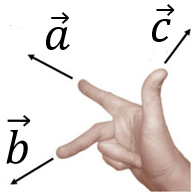
\includegraphics{rechterhandregel}
\end{image}
\captionof{figure}{De rechterhandregel}


\begin{remark}
    Een vector met zin in het blad wordt genoteerd met \(\otimes\). Een vector met zin uit het blad wordt genoteerd met \(\odot\).
\end{remark}

\end{document}
